\section{Learning Partial Orderings}

In this section we show how partial orderings on finite dimensional
spaces can be described as matrices, and give our algorithm for
learning such matrices from data.

\begin{figure*}
  \centering
  \begin{subfigure}[b]{0.3\textwidth}
    \scalebox{0.5}{
      %% Creator: Inkscape inkscape 0.48.0, www.inkscape.org
%% PDF/EPS/PS + LaTeX output extension by Johan Engelen, 2010
%% Accompanies image file 'cone.pdf' (pdf, eps, ps)
%%
%% To include the image in your LaTeX document, write
%%   \input{<filename>.pdf_tex}
%%  instead of
%%   \includegraphics{<filename>.pdf}
%% To scale the image, write
%%   \def\svgwidth{<desired width>}
%%   \input{<filename>.pdf_tex}
%%  instead of
%%   \includegraphics[width=<desired width>]{<filename>.pdf}
%%
%% Images with a different path to the parent latex file can
%% be accessed with the `import' package (which may need to be
%% installed) using
%%   \usepackage{import}
%% in the preamble, and then including the image with
%%   \import{<path to file>}{<filename>.pdf_tex}
%% Alternatively, one can specify
%%   \graphicspath{{<path to file>/}}
%% 
%% For more information, please see info/svg-inkscape on CTAN:
%%   http://tug.ctan.org/tex-archive/info/svg-inkscape

\begingroup
  \makeatletter
  \providecommand\color[2][]{%
    \errmessage{(Inkscape) Color is used for the text in Inkscape, but the package 'color.sty' is not loaded}
    \renewcommand\color[2][]{}%
  }
  \providecommand\transparent[1]{%
    \errmessage{(Inkscape) Transparency is used (non-zero) for the text in Inkscape, but the package 'transparent.sty' is not loaded}
    \renewcommand\transparent[1]{}%
  }
  \providecommand\rotatebox[2]{#2}
  \ifx\svgwidth\undefined
    \setlength{\unitlength}{259.341008pt}
  \else
    \setlength{\unitlength}{\svgwidth}
  \fi
  \global\let\svgwidth\undefined
  \makeatother
  \begin{picture}(1,0.63246843)%
    \put(0,0){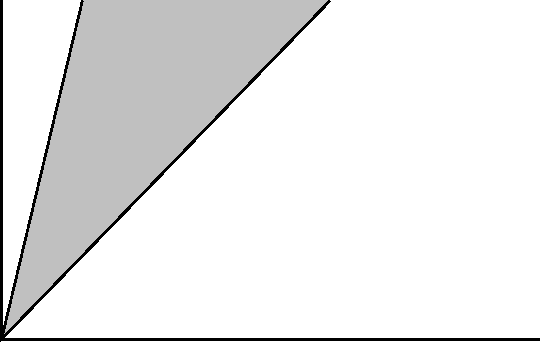
\includegraphics[width=\unitlength]{cone.pdf}}%
  \end{picture}%
\endgroup

    }
    \vspace{0.01cm}
    \caption{A cone}
    \label{fig:cone}
  \end{subfigure}
  \begin{subfigure}[b]{0.3\textwidth}
    \scalebox{0.5}{
      %% Creator: Inkscape inkscape 0.48.0, www.inkscape.org
%% PDF/EPS/PS + LaTeX output extension by Johan Engelen, 2010
%% Accompanies image file 'cones.pdf' (pdf, eps, ps)
%%
%% To include the image in your LaTeX document, write
%%   \input{<filename>.pdf_tex}
%%  instead of
%%   \includegraphics{<filename>.pdf}
%% To scale the image, write
%%   \def\svgwidth{<desired width>}
%%   \input{<filename>.pdf_tex}
%%  instead of
%%   \includegraphics[width=<desired width>]{<filename>.pdf}
%%
%% Images with a different path to the parent latex file can
%% be accessed with the `import' package (which may need to be
%% installed) using
%%   \usepackage{import}
%% in the preamble, and then including the image with
%%   \import{<path to file>}{<filename>.pdf_tex}
%% Alternatively, one can specify
%%   \graphicspath{{<path to file>/}}
%% 
%% For more information, please see info/svg-inkscape on CTAN:
%%   http://tug.ctan.org/tex-archive/info/svg-inkscape

\begingroup
  \makeatletter
  \providecommand\color[2][]{%
    \errmessage{(Inkscape) Color is used for the text in Inkscape, but the package 'color.sty' is not loaded}
    \renewcommand\color[2][]{}%
  }
  \providecommand\transparent[1]{%
    \errmessage{(Inkscape) Transparency is used (non-zero) for the text in Inkscape, but the package 'transparent.sty' is not loaded}
    \renewcommand\transparent[1]{}%
  }
  \providecommand\rotatebox[2]{#2}
  \ifx\svgwidth\undefined
    \setlength{\unitlength}{259pt}
  \else
    \setlength{\unitlength}{\svgwidth}
  \fi
  \global\let\svgwidth\undefined
  \makeatother
  \begin{picture}(1,0.71832129)%
    \put(0,0){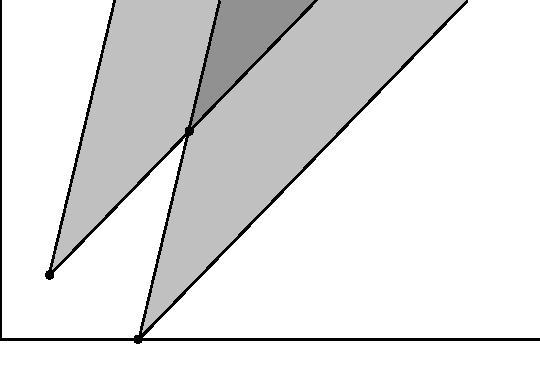
\includegraphics[width=\unitlength]{cones.pdf}}%
    \put(0.0289539,0.14386651){\color[rgb]{0,0,0}\makebox(0,0)[lb]{\smash{$u$}}}%
    \put(0.20731187,0.01815878){\color[rgb]{0,0,0}\makebox(0,0)[lb]{\smash{$v$}}}%
    \put(0.32271158,0.41831799){\color[rgb]{0,0,0}\makebox(0,0)[lb]{\smash{$u\lor v$}}}%
  \end{picture}%
\endgroup

    }
    \caption{Cone join}
    \label{fig:join}
  \end{subfigure}
  \begin{subfigure}[b]{0.3\textwidth}
    \scalebox{0.7}{
      %% Creator: Inkscape inkscape 0.48.0, www.inkscape.org
%% PDF/EPS/PS + LaTeX output extension by Johan Engelen, 2010
%% Accompanies image file 'basis.pdf' (pdf, eps, ps)
%%
%% To include the image in your LaTeX document, write
%%   \input{<filename>.pdf_tex}
%%  instead of
%%   \includegraphics{<filename>.pdf}
%% To scale the image, write
%%   \def\svgwidth{<desired width>}
%%   \input{<filename>.pdf_tex}
%%  instead of
%%   \includegraphics[width=<desired width>]{<filename>.pdf}
%%
%% Images with a different path to the parent latex file can
%% be accessed with the `import' package (which may need to be
%% installed) using
%%   \usepackage{import}
%% in the preamble, and then including the image with
%%   \import{<path to file>}{<filename>.pdf_tex}
%% Alternatively, one can specify
%%   \graphicspath{{<path to file>/}}
%% 
%% For more information, please see info/svg-inkscape on CTAN:
%%   http://tug.ctan.org/tex-archive/info/svg-inkscape

\begingroup
  \makeatletter
  \providecommand\color[2][]{%
    \errmessage{(Inkscape) Color is used for the text in Inkscape, but the package 'color.sty' is not loaded}
    \renewcommand\color[2][]{}%
  }
  \providecommand\transparent[1]{%
    \errmessage{(Inkscape) Transparency is used (non-zero) for the text in Inkscape, but the package 'transparent.sty' is not loaded}
    \renewcommand\transparent[1]{}%
  }
  \providecommand\rotatebox[2]{#2}
  \ifx\svgwidth\undefined
    \setlength{\unitlength}{188.26408691pt}
  \else
    \setlength{\unitlength}{\svgwidth}
  \fi
  \global\let\svgwidth\undefined
  \makeatother
  \begin{picture}(1,0.56574361)%
    \put(0,0){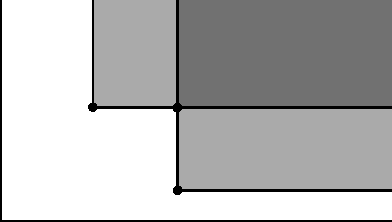
\includegraphics[width=\unitlength]{basis.pdf}}%
    \put(0.51254452,0.04251166){\color[rgb]{0,0,0}\makebox(0,0)[lb]{\smash{$u$}}}%
    \put(0.20261773,0.29920129){\color[rgb]{0,0,0}\makebox(0,0)[lb]{\smash{$v$}}}%
    \put(0.47721337,0.24375471){\color[rgb]{0,0,0}\makebox(0,0)[lb]{\smash{$u\lor v$}}}%
  \end{picture}%
\endgroup

    }
    \vspace{0.01cm}
    \caption{Basis cones}
    \label{fig:basis}
  \end{subfigure}
  \caption{A cone $C$ defining a lattice ordering on the two
    dimensional vector space in the plane (\subref{fig:cone}) and the
    join of two elements $u$ and $v$ (\subref{fig:join}). The shaded
    areas are $u + C$ and $v + C$. The basis associated with a vector
    space defines an ordering (\subref{fig:basis}); in this case, the
    basis is that defined by the $x$ and $y$ axes.}
\end{figure*}

A \textbf{cone} is a subset $C$ of a vector space satisfying
\begin{itemize}
\item $C + C \subseteq C$
\item $\alpha C \subseteq C$ for all $\alpha \ge 0$
\item $C \cap (-C) = \{0\}$
\end{itemize}
If $V$ is a partially ordered vector space, then the set $V^+ = \{v
\in V : v \ge 0\}$ is a cone, called the \textbf{positive
  cone}. Conversely, given any cone $C$ for a vector space $V$, we can
define a partial ordering on $V$ by $u \le v$ iff $v - u \in C$.

Given a countable set $U = \{u_1, u_2, \ldots\}$ of vectors, the cone
generated by $U$ is the set $C_U = \{v : v = \sum_i \alpha_i u_i\}$ for
some $\alpha_i \ge 0$.

\subsection{Matrices as Orderings}

\begin{proposition}[Partial Orderings Defined by Linear Operators]
  Let $A$ be a vector space and $B$ a partially ordered vector space,
  and let $M$ be a linear function from $A$ to $B$. Define an ordering
  on $A$ by $u\le v$ if and only if $Mu \le Mv$. Then $A$ is a
  partially ordered vector space under this ordering.
\end{proposition}

\begin{proof}
If $u \le v$ then $M(u + z) = Mu + Mz \le Mv + Mz = M(v +
z)$ so $u + z \le v + z$. Similarly, $M(\alpha u) = \alpha Mu
\le\alpha Mv = M(\alpha v)$ so $\alpha u \le \alpha v$ for
$\alpha \ge 0$.
\end{proof}

In particular, if we take $A = \R^n$ and $B = \R^m$ then $M$ is an $n$
by $m$ matrix. If we take the ordering for $A$ from Example
\ref{example:finite} then $u\le v$ if and only if $(Mu)_i \le (Mv)_i$
for all $i$.

\subsection{Learning Algorithm}

\begin{algorithm}
\caption{Cone Learning by Gradient Descent}\label{algorithm:cone}
\begin{algorithmic}
  \Procedure{LearnCone}{$V, \mathbf{c}, d$}
  \State $M \gets$ \Call{RandMatrix}{d}
  \State $\alpha \gets \alpha_0$
  \Loop
    \State $M' \gets$ \Call{Gradient}{$V, \mathbf{c}, M$}
    \Loop
      \State $N \gets M - \alpha M'$
      \State $N' \gets$ \Call{Gradient}{$V, \mathbf{c}, N$}
      \If{$\|N'\|_1 < \|M'\|_1$}
        \State \textbf{break}
      \EndIf
      \State $\alpha \gets \alpha/2$
      \If{$\alpha < \alpha_t$}
        \State \textbf{return} $M$
      \EndIf
    \EndLoop
    \State $M \gets N$
    \State $\alpha \gets 1.2\alpha$
  \EndLoop
  \EndProcedure
  \\
  \Procedure{Gradient}{$V, \mathbf{c}, M$}
  \State $A \gets MV$
  \State $B \gets$ \Call{Project}{$A, \mathbf{c}$}
  \State \textbf{return} $(A - B)V^T$
  \EndProcedure
  \\
  \Procedure{Project}{$U, \mathbf{c}$}
  \For{each column vector $\mathbf{u}_i$ in $U$}
    \If{$c_i = 1$}
      \State $\mathbf{u}_i \gets (\mathbf{u}_i)^+$
    \Else
      \State $m \gets \min(\mathbf{u}_i)$
      \If{$m > -0.1$}
        \State $j' \gets \argmin_j{(\mathbf{u}_i)_j}$
        \State $(\mathbf{u}_i)_j \gets -0.1$
      \EndIf
    \EndIf
  \EndFor
  \State \textbf{return} $U$
  \EndProcedure
\end{algorithmic}
\end{algorithm}

In this section we describe our learning algorithm (Algorithm
\ref{algorithm:cone}). Our approach is inspired by that of
\newcite{Hoyer:04}, who describes an approach for learning sparse
non-negative matrix factorisations based on gradient descent. Although
our goal and implementation is unique, we are able to adapt the
gradient descent technique to our ends. Our algorithm is implemented
in Python and is open sourced under the MIT license.\footnote{Location
  withheld to preserve anonymity.}

Let $\mathbf{v}$ be an instance vector and $c \in \{0,1\}$ the class value of
the instance, where 0 indicates the instance is not positive, and 1
indicates that it is positive. Our goal is to learn a matrix $M$ such
that $M\mathbf{v} \ge 0$ if and only if $c = 1$, for as many instance vectors
as possible.

Let $V$ be the matrix whose columns are the instance vectors in the
training data, and let $\mathbf{c}$ be the binary vector of
corresponding class values.

We also need to fix the parameter $d$, the dimensionality of the space
describing the partial ordering. Then $M$ is a $d$ by $n$ matrix,
where $n$ is the number of instance features, i.e.~the dimensionality
of the instance vectors $\mathbf{v}$. We initialise this to a random
matrix with values in $[-1,1]$, and then begin the loop in which the
gradient descent occurs. The gradient $M'$ is computed by projecting
$MV$ such the resulting matrix satisfies the goal of making all
positive instances in the training data positive ($\mathbf{u}^+$ is
the vector with all negative components of $\mathbf{u}$ set to zero)
and all non-positive instances are not positive. The gradient is then
estimated by multiplying the difference between $MV$ and its
projection with $V^T$.

The parameter $\alpha$ is tuned using a heuristic from the
implementation of \newcite{Hoyer:04}, and determines how far we move
in the direction of the gradient in each loop. We initialise $\alpha$
to $\alpha_0$ and stop when $\alpha$ is smaller than the threshold
$\alpha_t$.

\subsection{Avoiding Local Minima}

We found in our initial experiments, particularly with low-dimensional
data, that the gradient descent algorithm gets stuck in local
minima. To mitigate this, we do a few iterations of the gradient
descent algorithm from a number of different initial matrices, and
choose the one that works the best on the training data. We then do a
gradient descent until convergence on this best performing matrix.

\subsection{Handling Noisy Data}

We also found in testing that the algorithm could not cope well with
noisy data; in particular if a data point is marked as positive but is
actually in the negation of the cone, this prevents the algorithm from
finding the optimal solution. To get around this, we relaxed the
projection algorithm so that it only affects those that are already
closest to being correct. This effectively gives us automatic outlier
detection, where the proportion of outliers that should not be
adjusted in the projection is specified as a parameter.

